% !TeX spellcheck = en_US
\chapter{Testing}
\section*{Languages and Frameworks}
In order to test our system, we need to use a tool to create a \textit{virtual network} inside our machine: we used \texttt{mininet}\footnote{http://mininet.org/}, 
exploiting the \texttt{python2} APIs. To simulate input from an external application we also used a python2 library, called \texttt{requests}\footnote{https://docs.python-requests.org/en/latest/},
which is able to act like an HTTP client.\
Given that our developement environment is inside a virtual machine, we will keep the number of virtual devices relatively small, in order to not
overload the VM resources.

\section*{Scenario}
We want to simulate a typical data center scenario with a single LAN, implemented in a \textit{Spine-Leaf} topology. This configuration
is widely used thanks to its easy scalability and sufficient redundancy.
\begin{figure}[h]
    \centering
    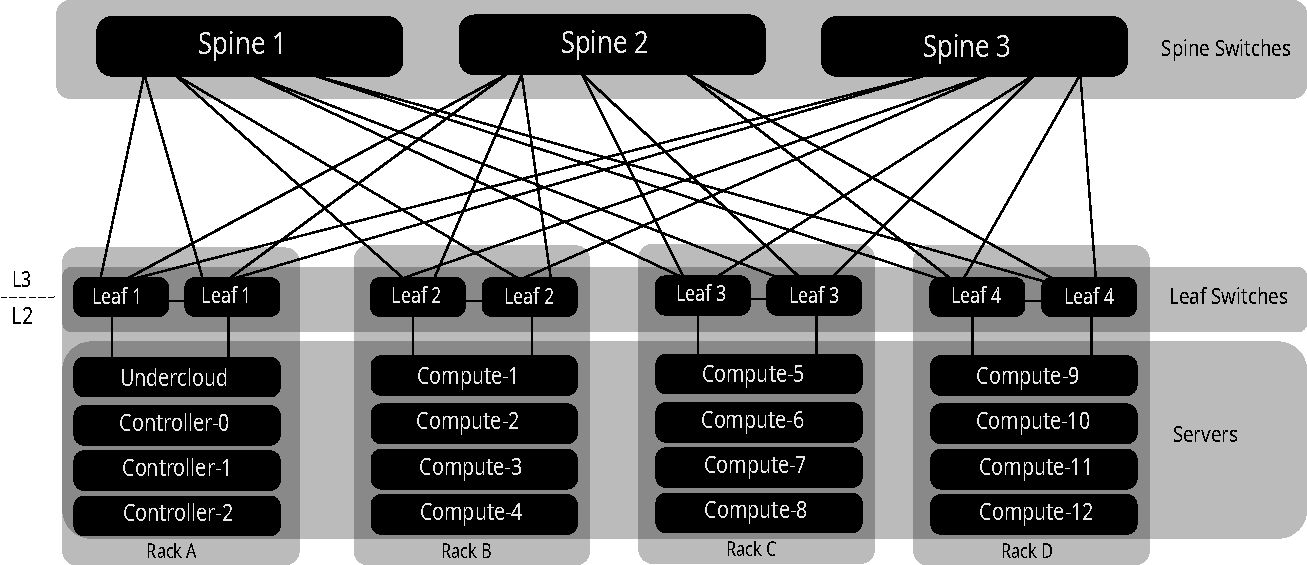
\includegraphics[width=0.90\textwidth]{img/spine_leaf.pdf}
    \caption{example of \textit{spine-leaf} topology}
\end{figure}

\section{Link Failure Test}
\noindent Using \texttt{mininet}, we can also simulate an episode of link failure, in order to test the system behaviour in this specific case. The system is able to recompute a functional path between two host and use it to forward packets.

\noindent In order to perform this test we use a spine leaf network with 2 spines and 3 leaf, each leaf has two hosts connected to it. The links of the network can be seen in figure \ref{img:links}

\begin{figure}[h]
	\centering
	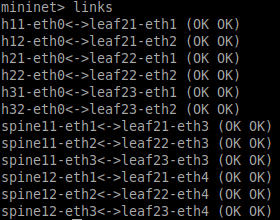
\includegraphics[width=0.50\textwidth]{img/links.png}
	\caption{Links of the spine leaf network}
	\label{img:links}
\end{figure}

\noindent To prove that the system is capable of handling a link failure we will establish an intent, use wireshark to sniff the traffic on the interfaces of the spines and see what happens when a link failure takes place and how the traffic is redirected.

\noindent The first thing to do is obviously to start the floodligh controller and the network\footnote{through the script scripts/start\_only\_spine\_topo.py}, then we establish an intent between the host11 (connected to leaf21) and the host21 (connected to leaf22). In order to check the connectivity we use wireshark on spine11-eth1 (the interface that connects leaf21 with spine11) and spine12-eth1 (the interface that connects leaf21 with spine12) and we perform a ping between the two hosts to see what happens on these interfaces.

\begin{figure}[h]
\centering
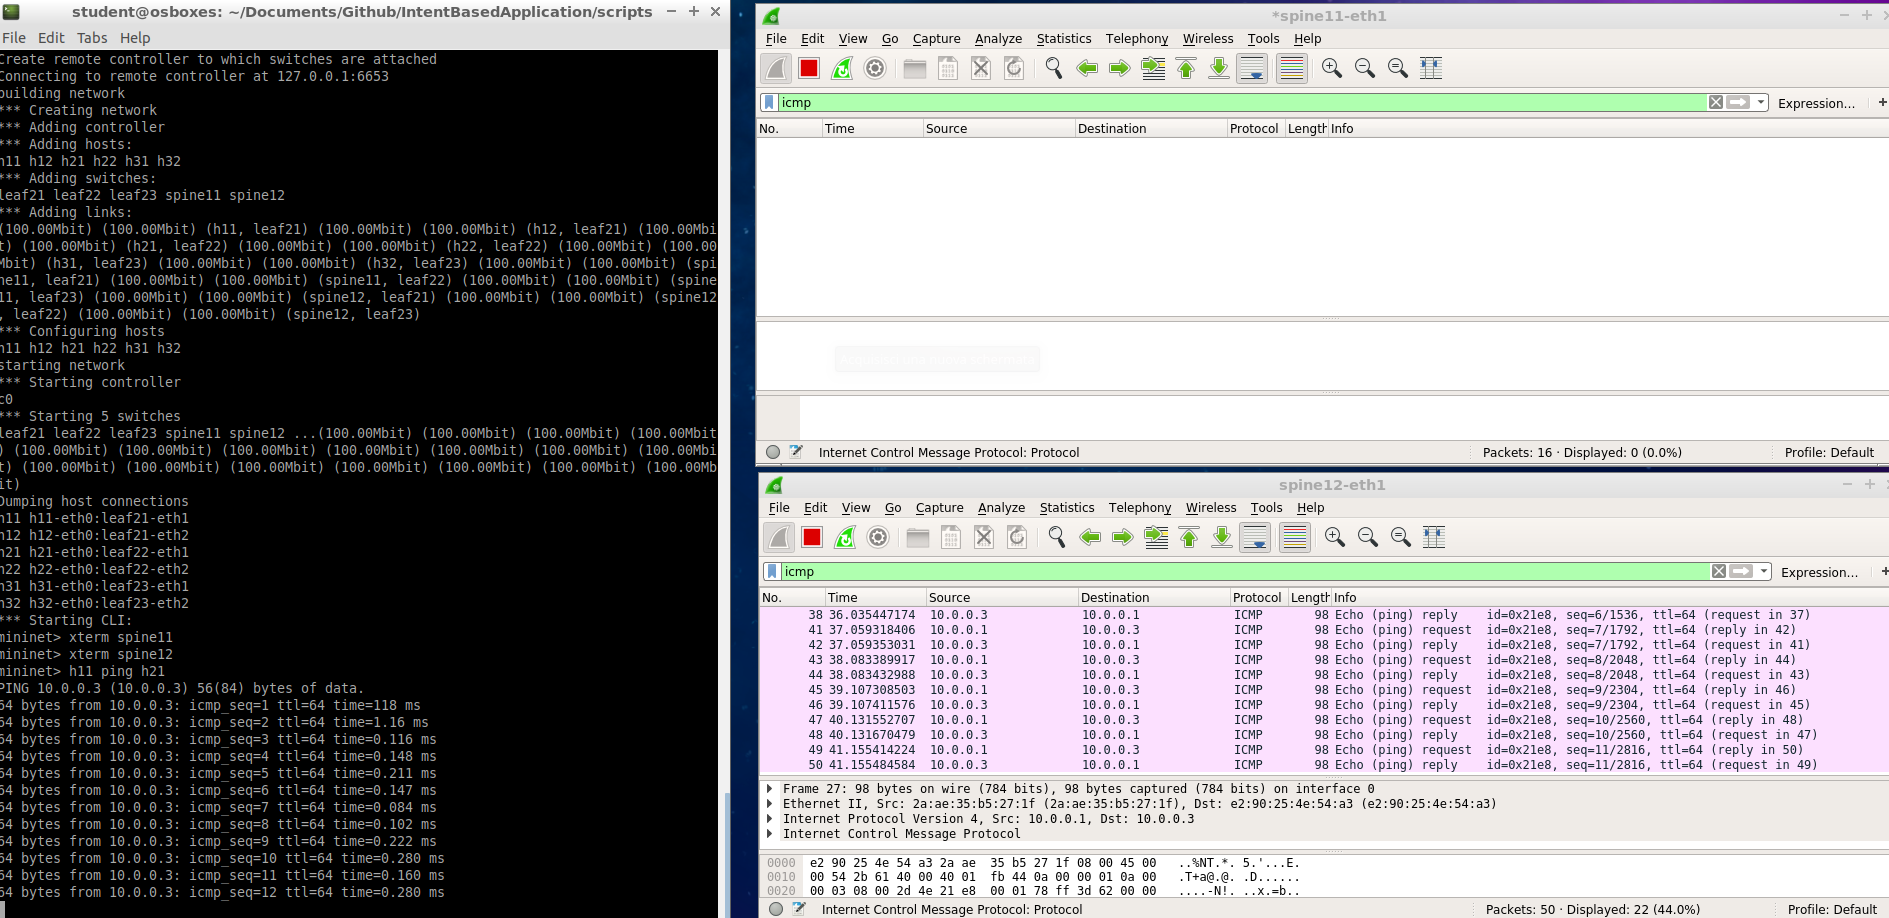
\includegraphics[width=1\textwidth]{img/ping1.png}
\caption{Ping between host11 and host21}
\label{img:ping1}
\end{figure}

\noindent As we can see in figure \ref{img:ping1} the ping is executed succesfully and the interface spine12-eth1 is used to forward the traffic. Now we put down the link between leaf21 and spine12, so the interface spine12-eth1 is now down (see figure \ref{img:linkdown}).

\begin{figure}[h]
	\centering
	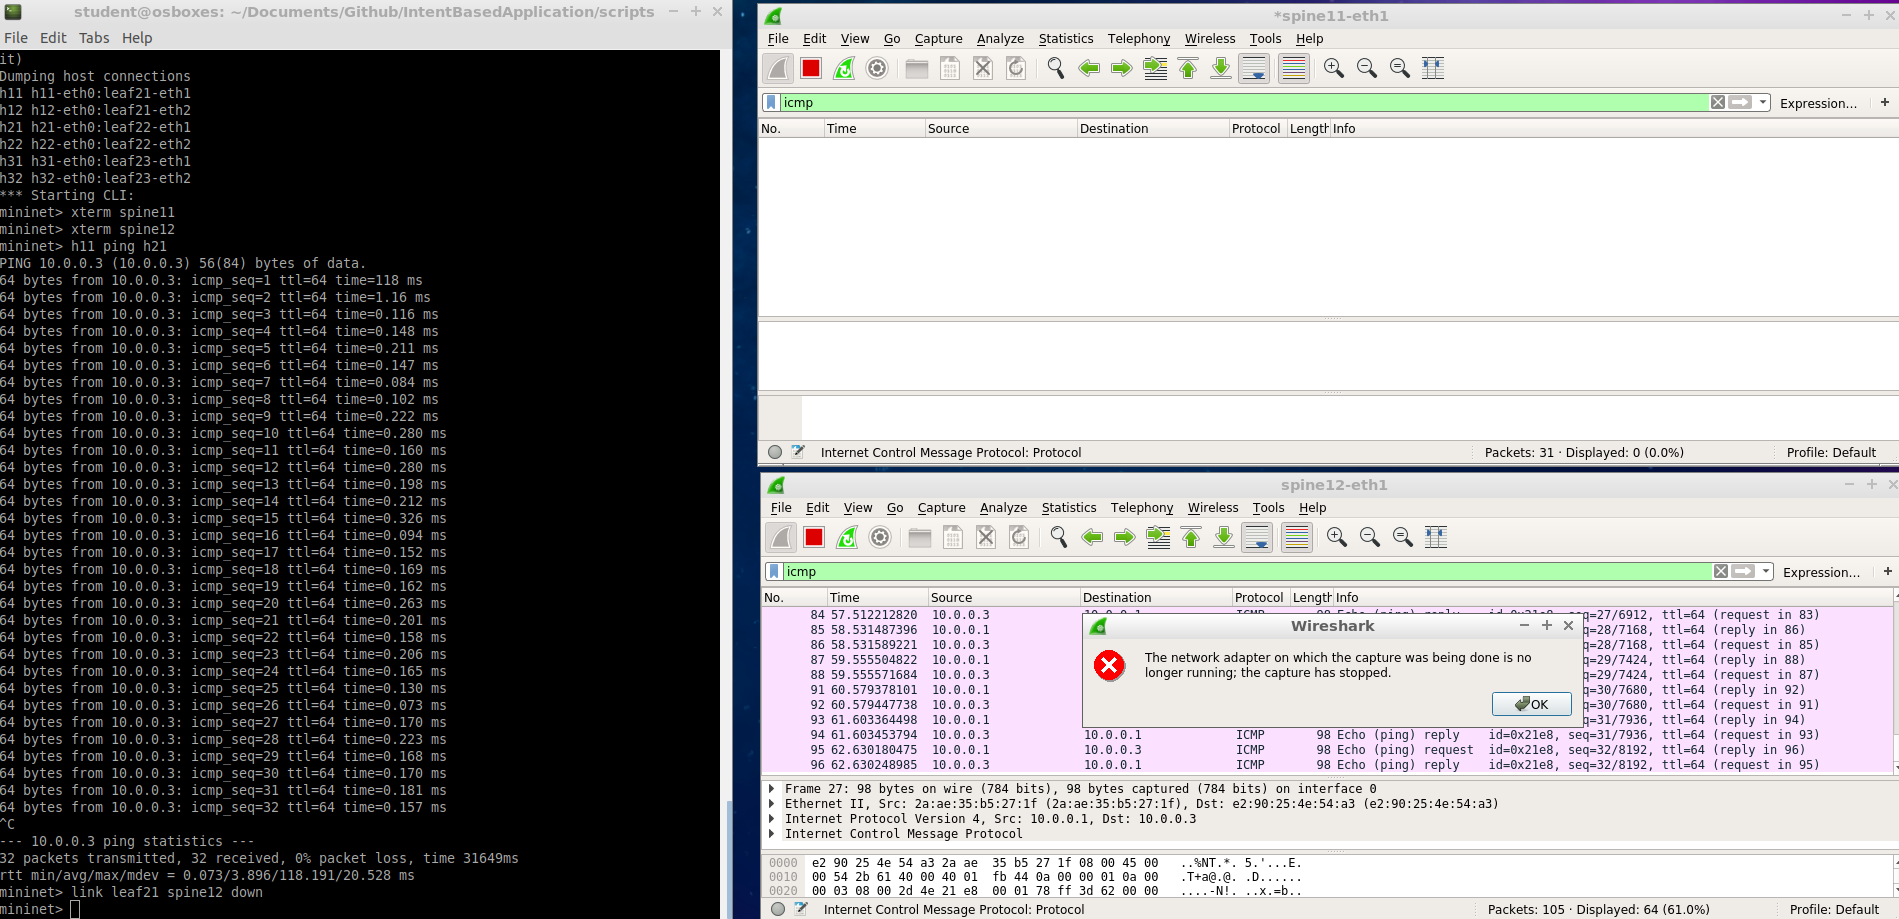
\includegraphics[width=1\textwidth]{img/linkdown.png}
	\caption{We put down the link between leaf21 and spine12}
	\label{img:linkdown}
\end{figure}

\noindent Then we perform another time the ping and we see that the interface spine11-eth1 is used to forward traffic (see figure \ref{img:failurehandler}).

\begin{figure}[h]
	\centering
	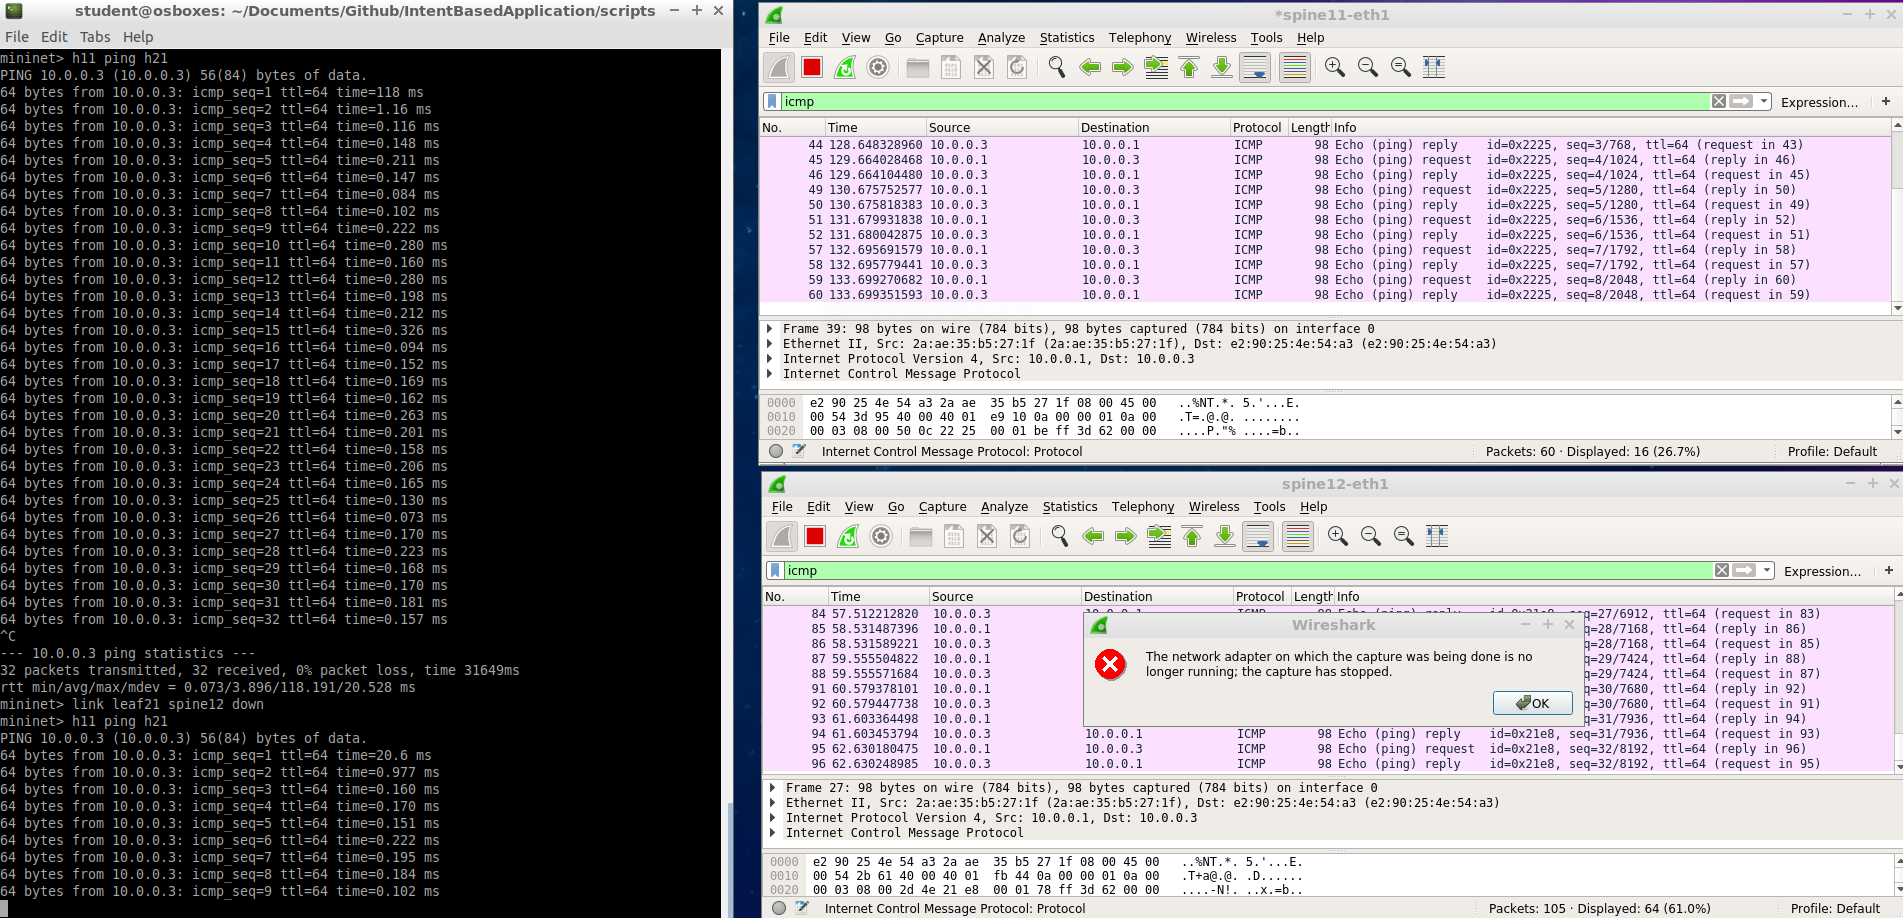
\includegraphics[width=1\textwidth]{img/failurehandler.png}
	\caption{Host11 now uses spine11-eth1 to perform the ping}
	\label{img:failurehandler}
\end{figure}

\noindent Thus we can state that at the beginning host11 used spine21 to communicate with host21 but when the link between leaf21 and spine21 failed (and so host11 cannot communicate anymore with spine21) host11 uses spine11 and so the intent continues to be valid. Hence the system is able to cope with a link failure.


\newpage
\section{Ping Latency}
In order to measure the network performance we will consider a fixed scenario with 2 spines, 3 leafs and 4 hosts for each leafs (i.e. 12 hosts in total);
for every host:
\begin{itemize}
    \item  we establish an intent with another random chosen one;
    \item  we start a ping session, measuring the \texttt{round trip time} of each packet
    \item  the session end when 10 ping are successfully exchanged, or the last timeout elapses
\end{itemize} 
\begin{figure}[h]
    \centering
    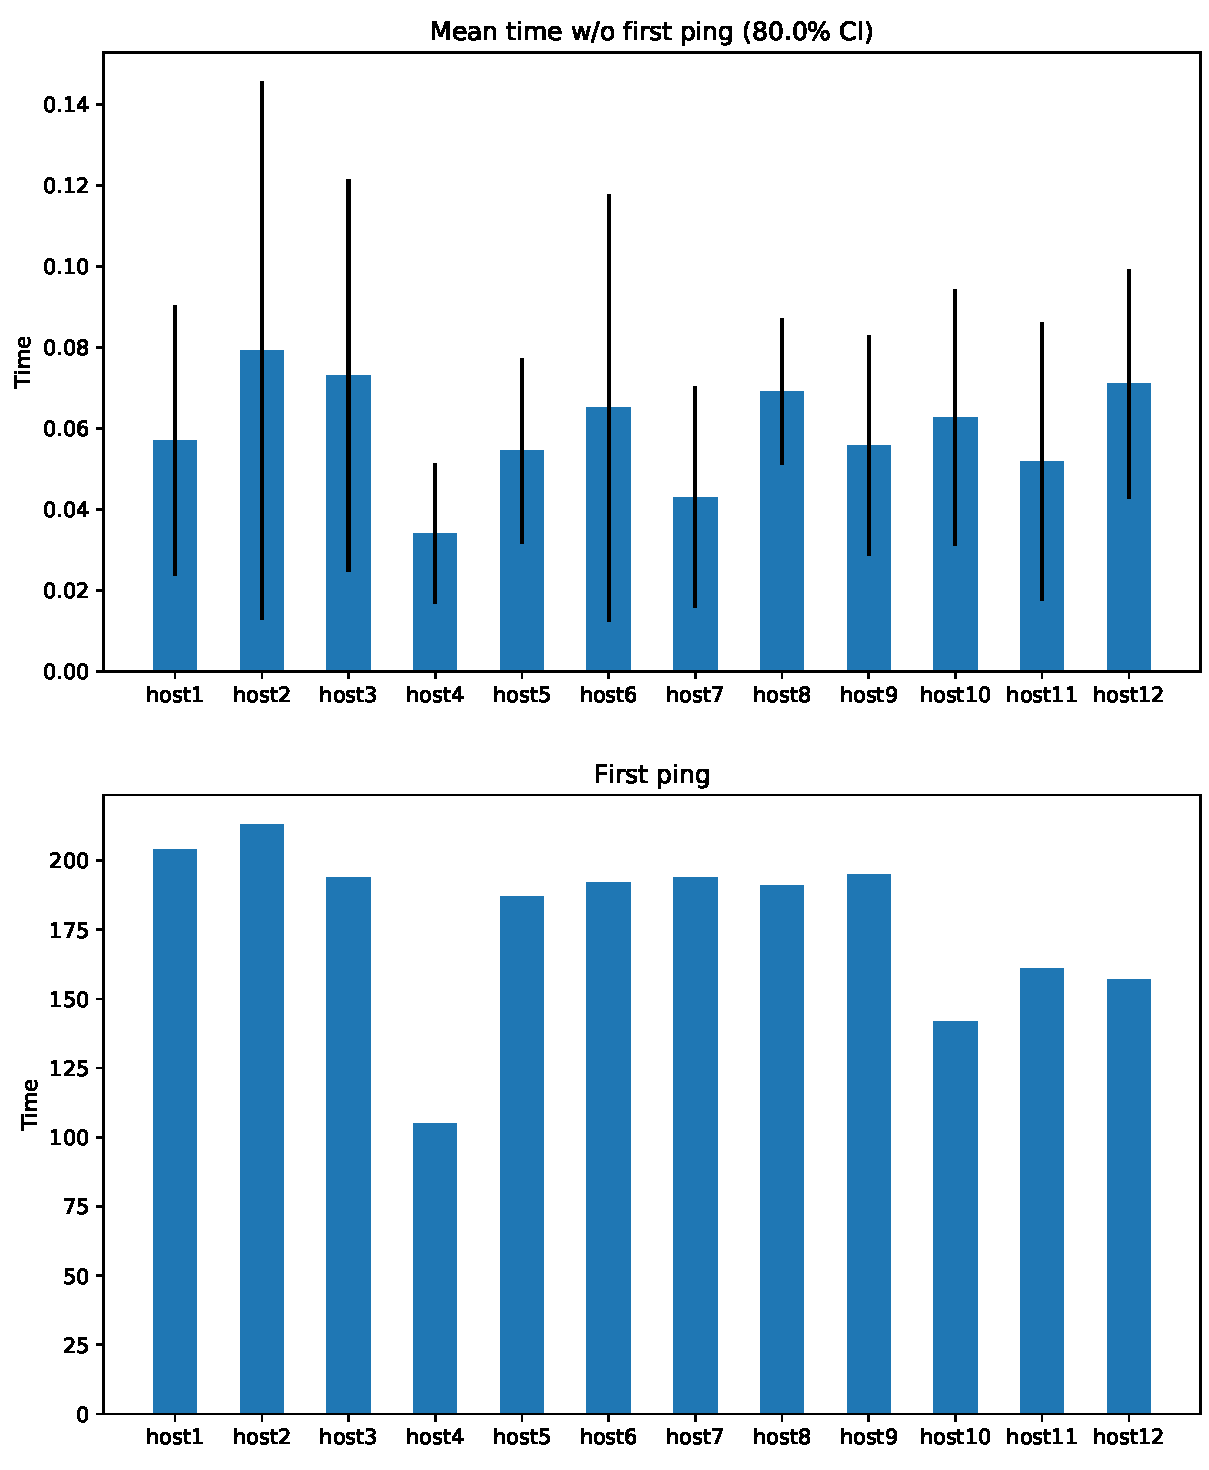
\includegraphics[width=.92\textwidth]{img/mean_ping_time.pdf}
    \caption{Ping times with 12 hosts}
    \label{img:perf1}
\end{figure}
First of all we monitor the number of \texttt{DESTINATION HOST UNREACHABLE} and \texttt{DUPLICATE}, those 2 parameters are equal to 0, confirming the correct
behaviour of the network.
The performance results (see figure \ref{img:perf1}) are consistent with our expectation:
\begin{itemize}
    \item the first ping is significantly slower than the others, because it is processed by the controller, triggering the route establishment;
    \item subsequent pings are very fast (<1 ms), because they don't have to traverse "real" network cables and because they are processed by the virtual switches and not by the controller.
\end{itemize}
\newpage
\begin{figure}[h]
    \centering
    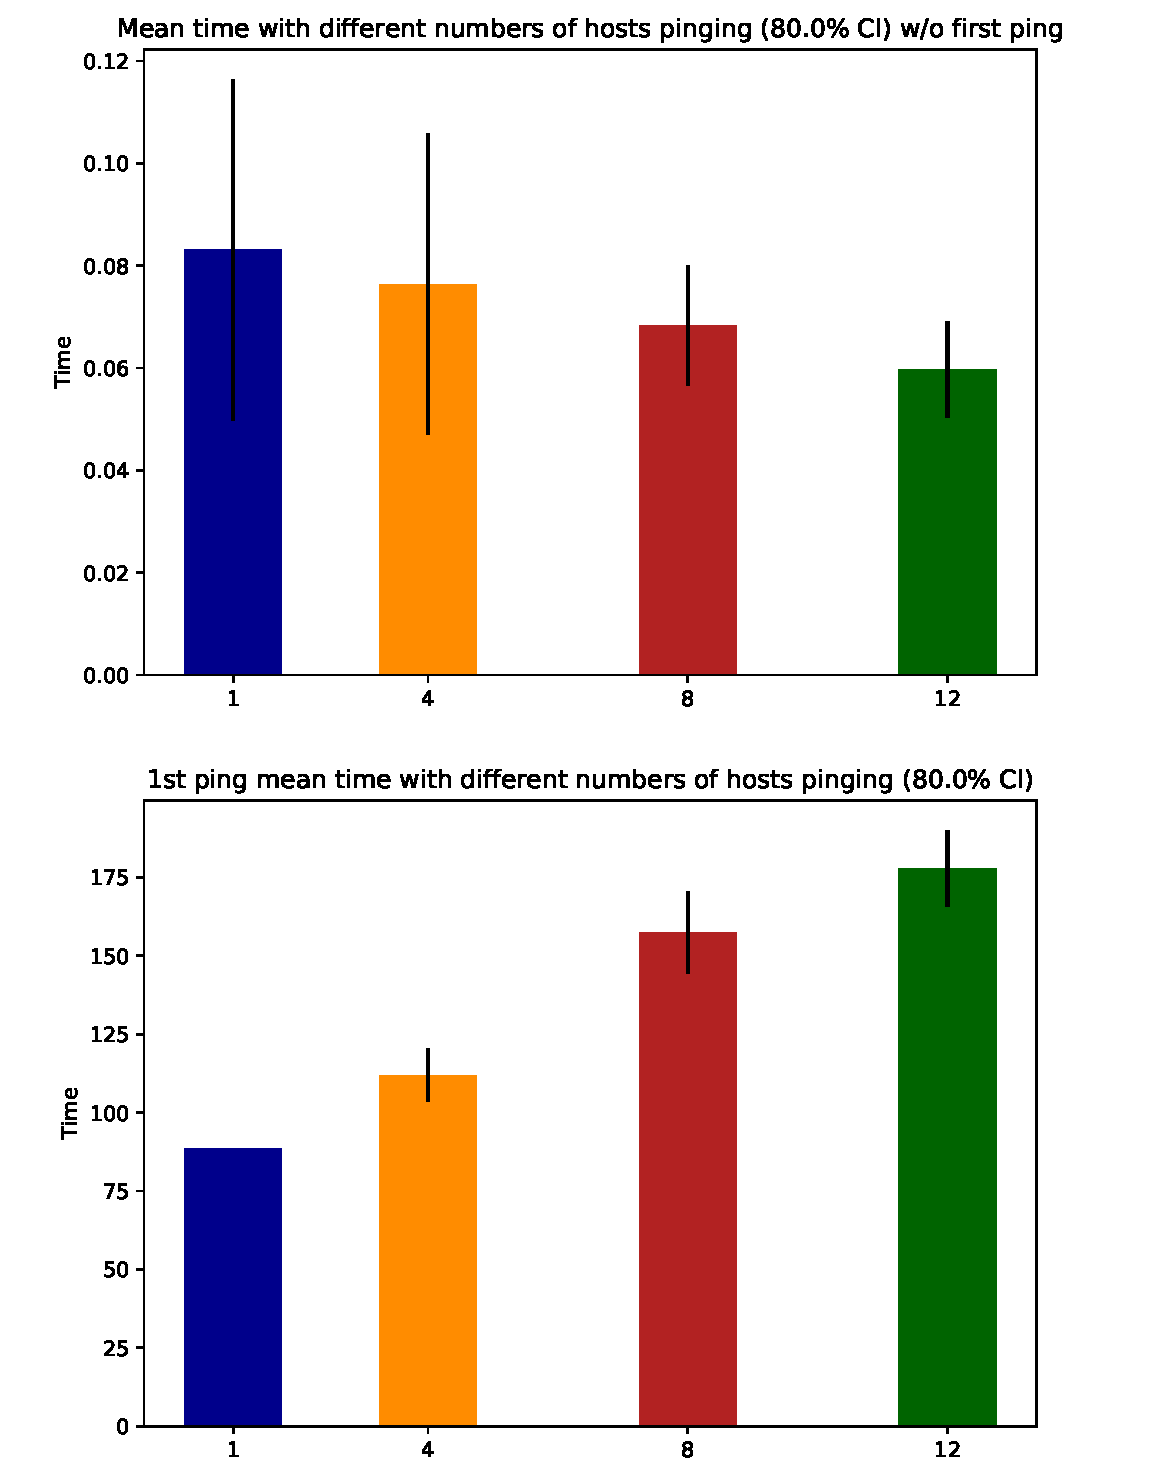
\includegraphics[width=.94\textwidth]{img/increasing_ping_time.pdf}
    \caption{Ping times with different loads}
    \label{img:perf2}
\end{figure}
\noindent We also tried to evaluate the elasticity of the network with increasing load of traffic (i.e. increasing number of host pinging at the same time) and the results of this tests can be seen in figure \ref{img:perf2}.\\
The time needed for the first ping to complete tends to increase with the amount of traffic meanwhile the time for the others pings remains pretty stable
(mind the confidence intervals). This is expected because route establishment is done by the controller in a centralized way (the requests will queue up);
once the route is established, switches will handle the traffic in a distributed manner, leading to optimal forwarding of traffic.